\documentclass{article}
\usepackage{graphicx} % Required for inserting images
\usepackage{amsmath}
\usepackage{amssymb}
\usepackage{amsthm}
\setlength{\parindent}{0pt}
\usepackage[dvipsnames]{xcolor}
\newcommand{\lra}{\ensuremath\longrightarrow}
\usepackage{caption}
\usepackage{subcaption}
\usepackage[section]{placeins}

\title{Final Project 320}
\author{Brookes Heil-Blackburn}
\date{April 2024}

\begin{document}

\maketitle

\section*{Euler Mascheroni Constant}
Let $H_n$ = $\sum_{k=1}^{n}$ $\frac{1}{k}$. Prove $ \lim_{n\to\infty}$ $H_n - ln(n) = \gamma$ exists and find a numeric approximation for $\gamma$.
\FloatBarrier
\section{Prove Existence of $\gamma$}
We will prove that for $H_n$ = $\sum_{k=1}^{n}$ $\frac{1}{k}$ there exists a value of convergence $\gamma$ = $ \lim_{n\to\infty}$ $H_n - ln(n)$. \\
$ln(n)=\int_{1}^{n} \frac{1}{x}dx$.\\
Let $S_n$ = $\sum_{k=1}^{n}$ $\frac{1}{k} - \int_{1}^{n} \frac{1}{x}dx$\\
We will show that this series is monotonically decreasing and bounded from below thus proving a convergence value exists.
\begin{center}
\FloatBarrier
\begin{figure}[htp]
    \centering
    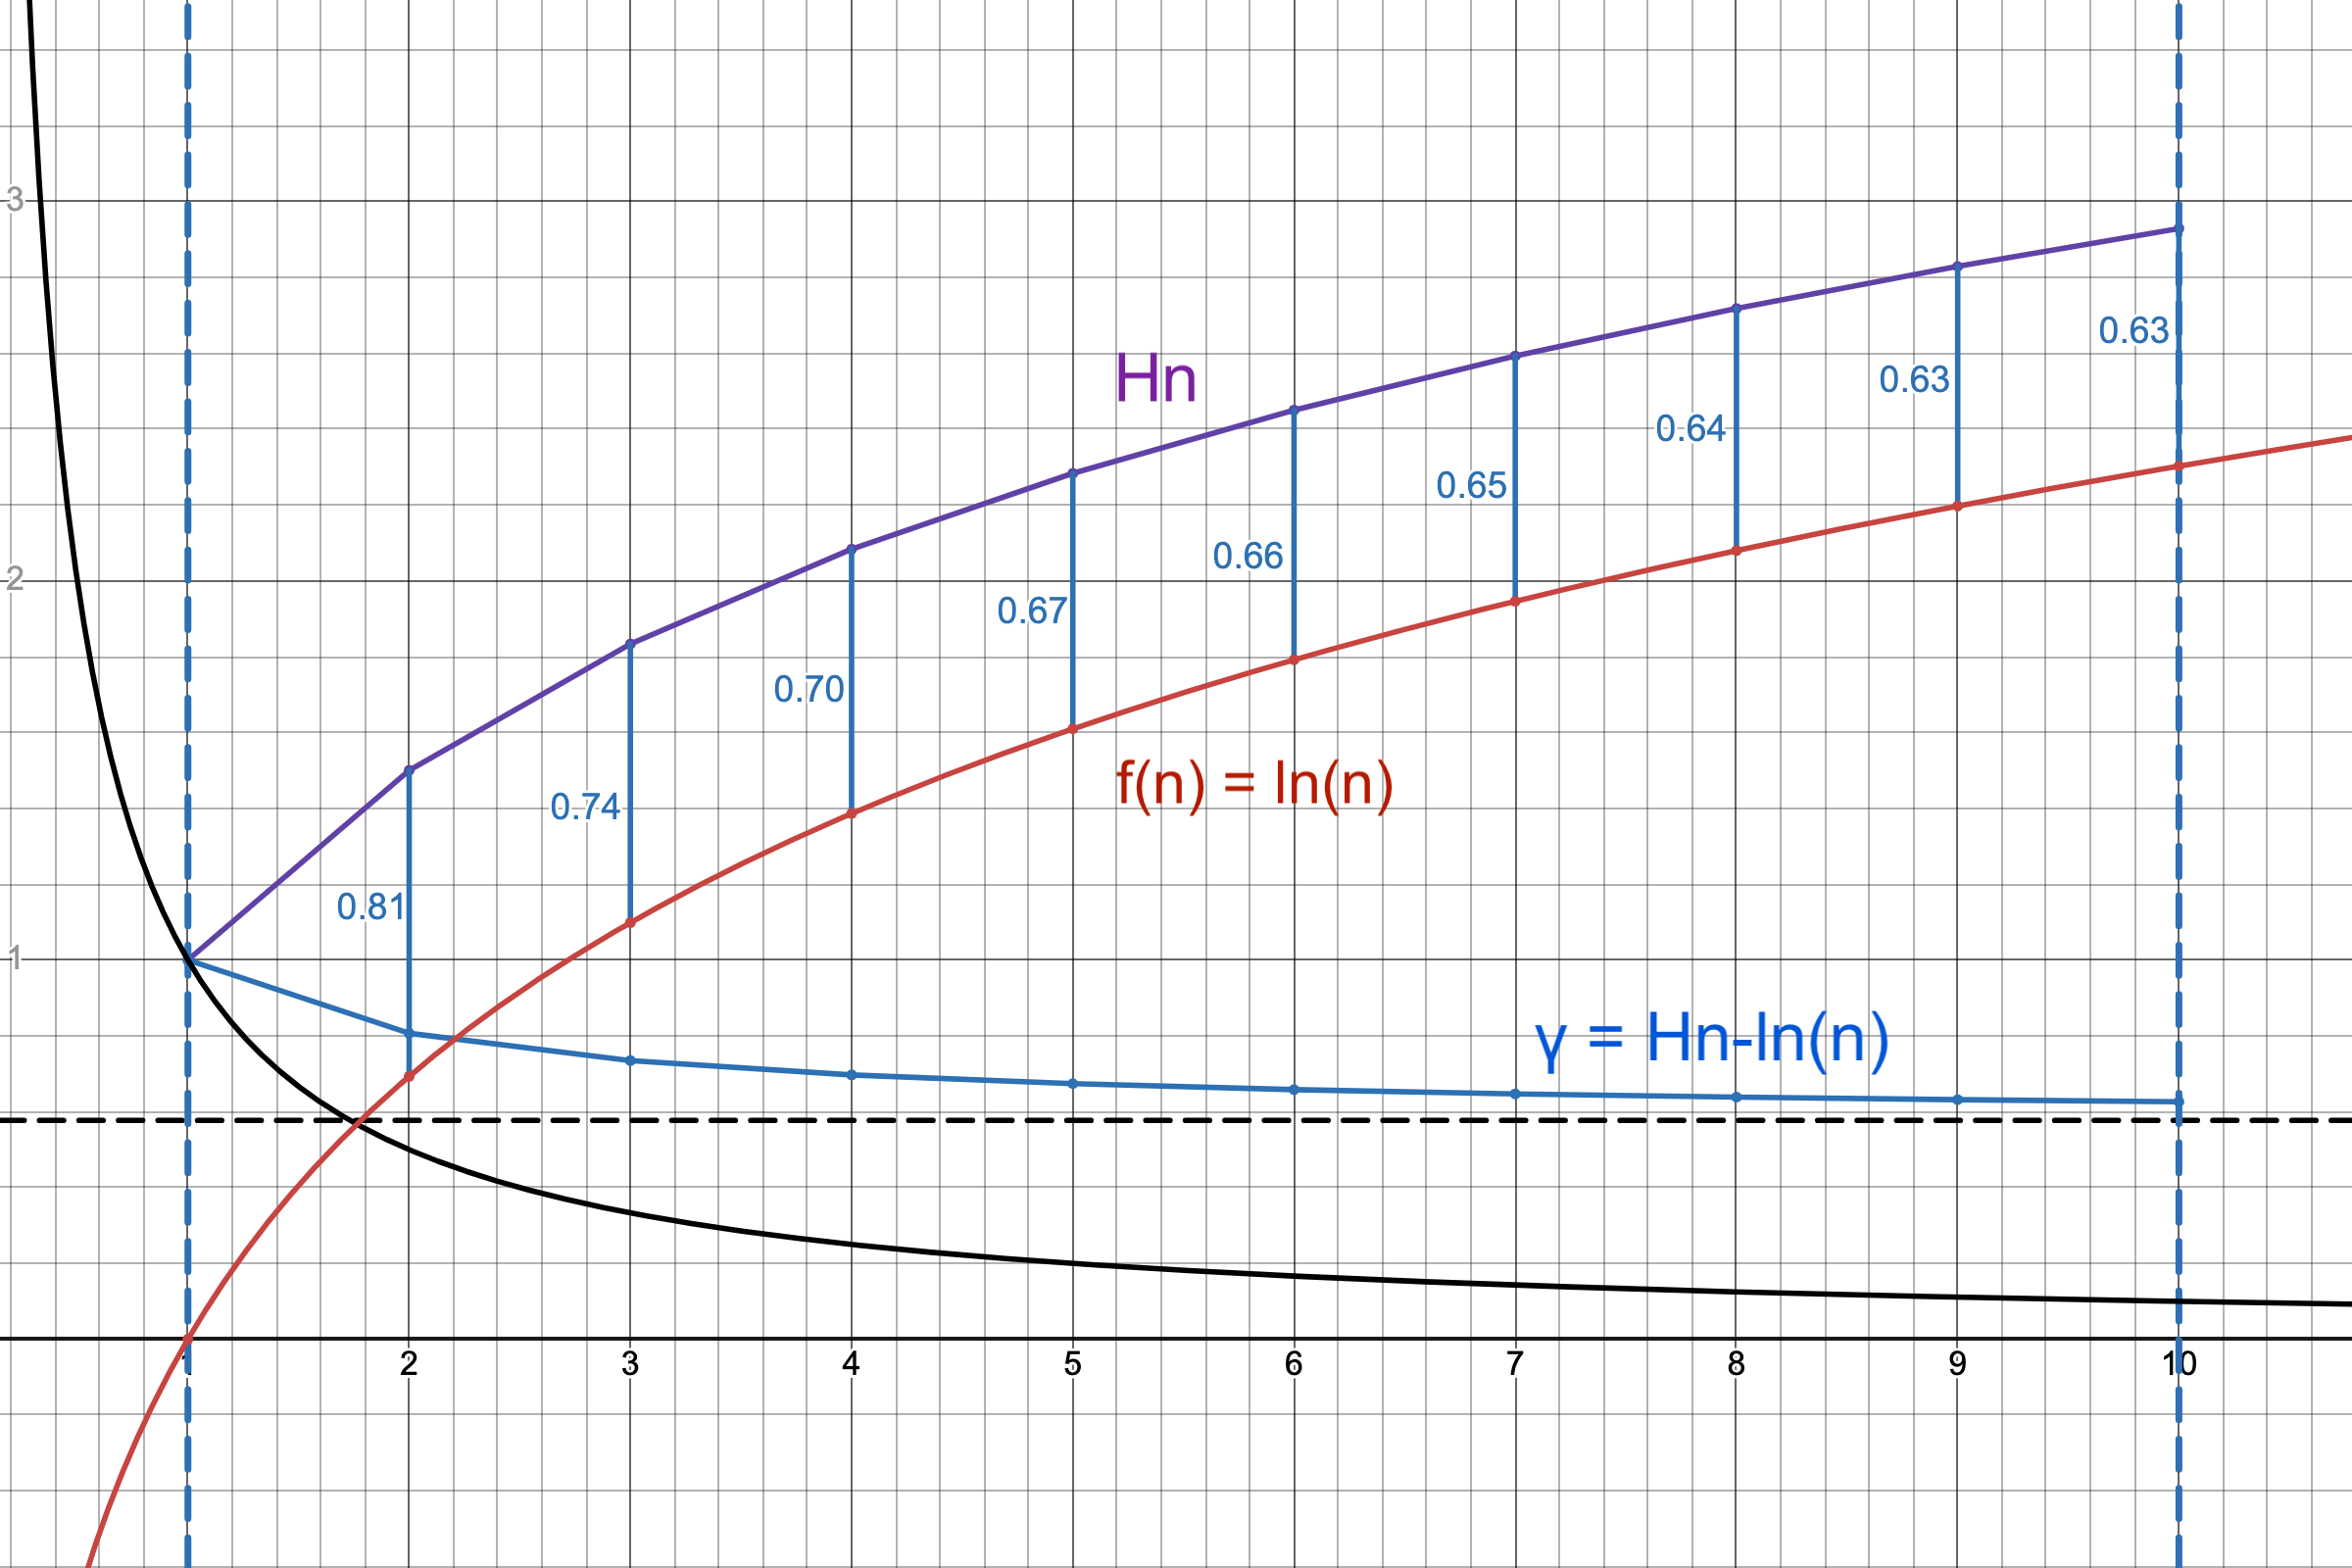
\includegraphics[scale=0.1]{simplified gamma.png}
    \caption{\textcolor{violet}{$H_n = \sum_{k=1}^{n}\frac{1}{k}$}, \textcolor{red}{$ln(n)$}, \textcolor{blue}{$\sum_{k=1}^{n}$ $\frac{1}{k} - \int_{1}^{n} \frac{1}{x}dx$}}
    \label{fig:galaxy}
\end{figure}
\end{center}
\FloatBarrier
\subsection{Show $S_n$ is Monotonically Decreasing}
We will start by showing that $S_n$ is monotonically decreasing.   We will prove that for all values of $n$, $S_n > S_{n+1}$. $S_n-S_{n+1}>0$\\
$S_n-S_{n+1}$:
$$=(\sum_{k=1}^{n}\frac{1}{k} - \int_{1}^{n} \frac{1}{x}dx)-(\sum_{k=1}^{n+1}\frac{1}{k} - \int_{1}^{n+1} \frac{1}{x}dx)$$
$$=(\sum_{k=1}^{n}\frac{1}{k}-\sum_{k=1}^{n+1}\frac{1}{k})+ (\int_{1}^{n+1} \frac{1}{x}dx-\int_{1}^{n} \frac{1}{x}dx)$$
$$=(\sum_{k=1}^{n}\frac{1}{k}-\sum_{k=1}^{n+1}\frac{1}{k})+(\int_{n}^{n+1} \frac{1}{x}dx$$
$$=((-1)(\frac{1}{n+1})+\int_{n}^{n+1} \frac{1}{x}dx)$$
\begin{center}
\begin{figure}[htp]
    \centering
    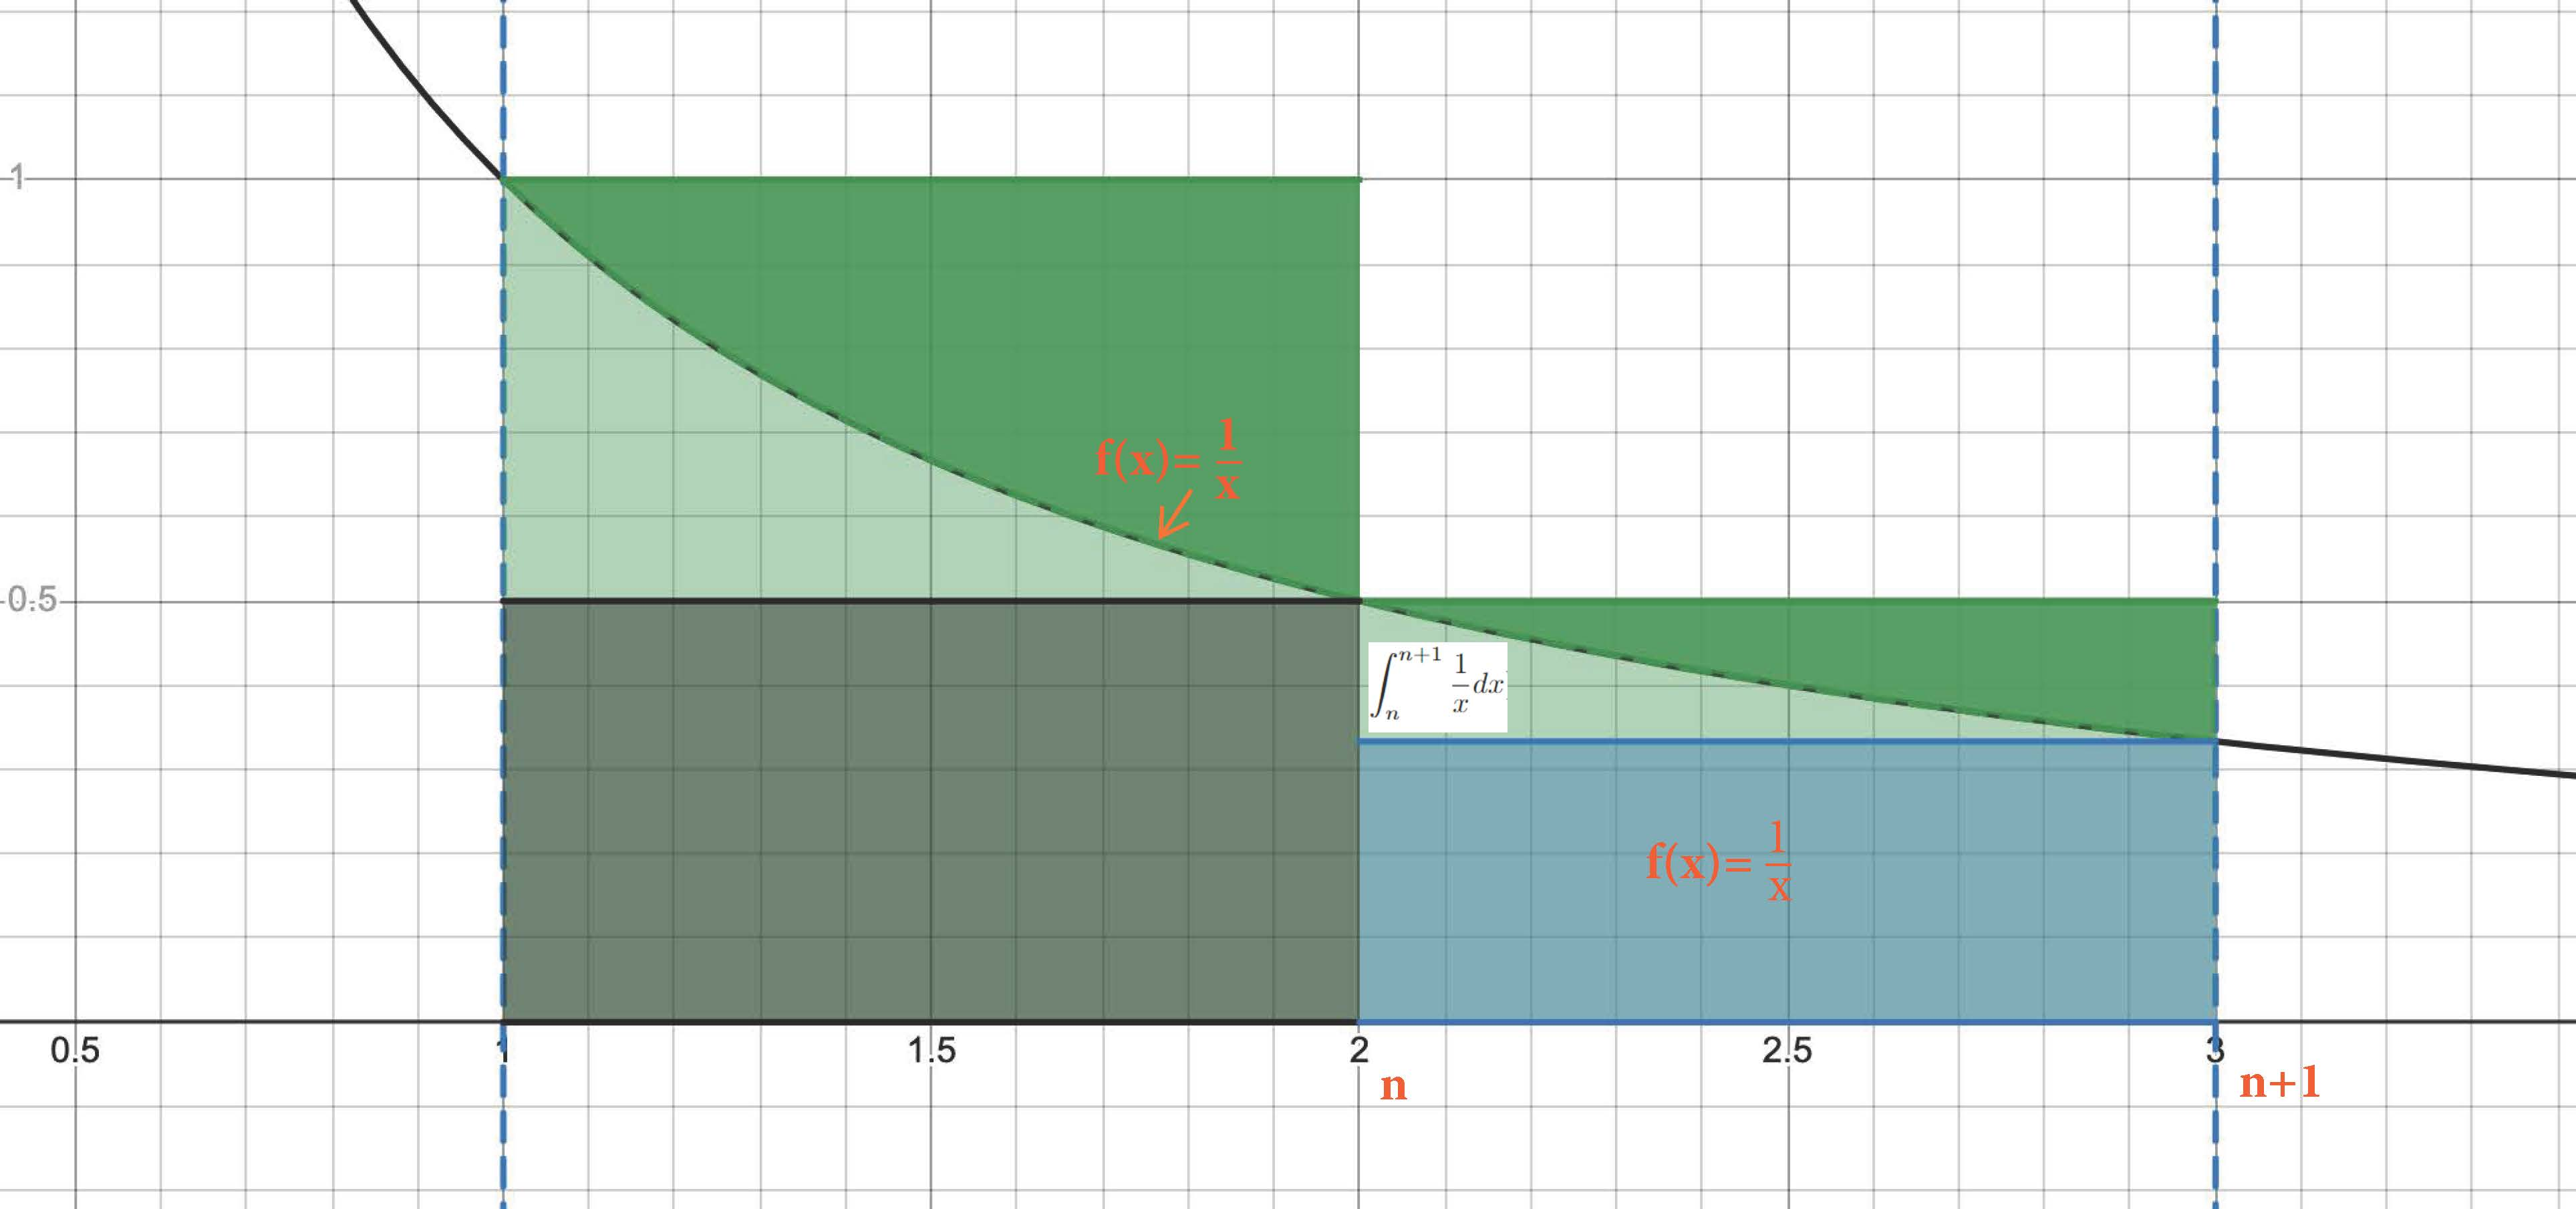
\includegraphics[scale=0.25]{n and n+1 zoomed in more rev1.jpg}
    \caption{\textcolor{Gray}{Integral $\int_n^{n+1} \frac{1}{x}dx > f(x)=\frac{1}{x}$}}
    \label{fig:Riemann Sums}
\end{figure}    
\end{center}
For a decreasing function, the right-hand Reimann sum from n to n+1 is less than the value of integral for n to n+1.
Subtracting the right-hand value of the function from the integral will result in a value greater than 0. 
Since $$S_n-S_{n+1}=((-1)(\frac{1}{n+1})+\int_{n}^{n+1} \frac{1}{x}dx)$$
and
$$0<((-1)(\frac{1}{n+1})+\int_{n}^{n+1} \frac{1}{x}dx)$$
we have shown that
$$0<S_n-S_{n+1}$$
This proves that $S_{n+1}<S_n$, and that the series is monotonically decreasing.
\FloatBarrier
\subsection{Lower Bound}
We will show that $0\leq S_n$ for all values of n.
$$S_n=(\sum_{k=1}^{n}\frac{1}{k} - \int_{1}^{n} \frac{1}{x}dx)$$
The left end point Riemann sum of a decreasing (in our case concave) function is always greater than the value of the area under the function. This shows that $0\leq S_n$.
\begin{figure}[htp]
    \centering
    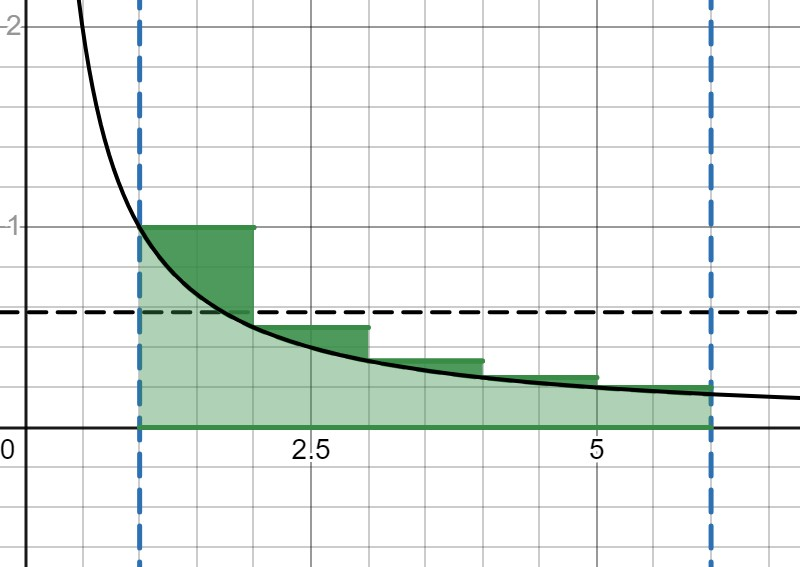
\includegraphics[scale=0.25]{Lower Bound Graph.jpg}
    \caption{\textcolor{gray}{Graphical Representation of Left-Hand Riemann Sums always greater than the value of the area under the function $\sum_{k=1}^{n}\frac{1}{k} \geq \int_{1}^{n} \frac{1}{x}dx)$.}}
    \label{fig:Riemann Sums}
\end{figure}  
\FloatBarrier
\subsection{Upper Bound}
Since $S_n$ is decreasing we know that $S_n<S_1$.  Where $S_1 = \sum_1^1 \frac{1}{1} - ln(1))=(1-0)=1$. We have shown $S_n$ is bounded above by 1. 
\begin{figure}[htp]
    \centering
    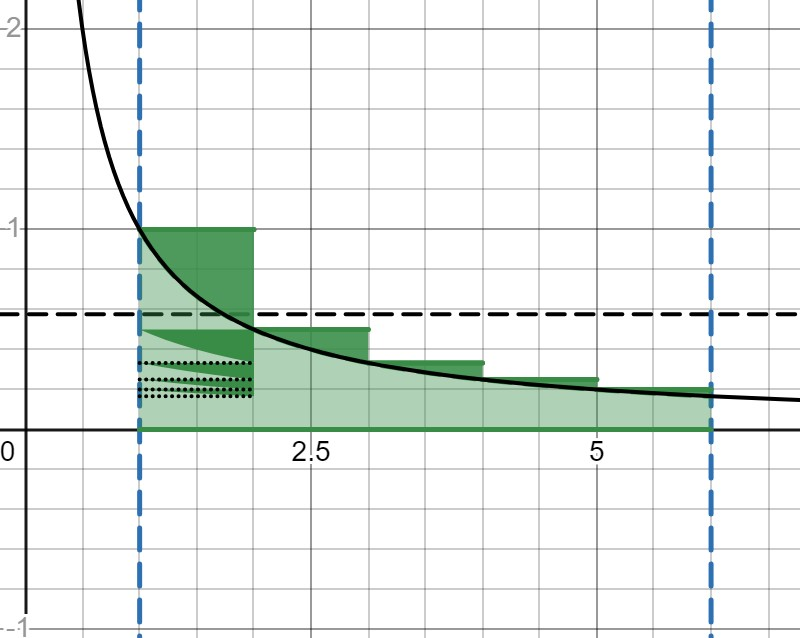
\includegraphics[scale=0.3]{Upper Bound Graph.jpg}
    \caption{\textcolor{gray}{Graphical Representation of $\sum_{k=1}^n(\frac{1}{n}-(ln(n+1)-ln(n))=\gamma$ (dark shaded areas) is bounded above by 1.}}
    \label{fig:Riemann Sums}
\end{figure} 
\FloatBarrier
\subsection{Summary of Existence}
We have shown that the series $S_n=\sum_{k=1}^n \frac{1}{k}-\int_1^n \frac{1}{x}dx$ is monotonically decreasing and bounded below. This implies that $H_n-ln(n)$ both exists and converges. We have also shown that $0 \leq S_n \leq 1$.
\FloatBarrier
\section{Estimate Value of $\gamma$}
\FloatBarrier
\begin{figure}[htp]
    \centering
    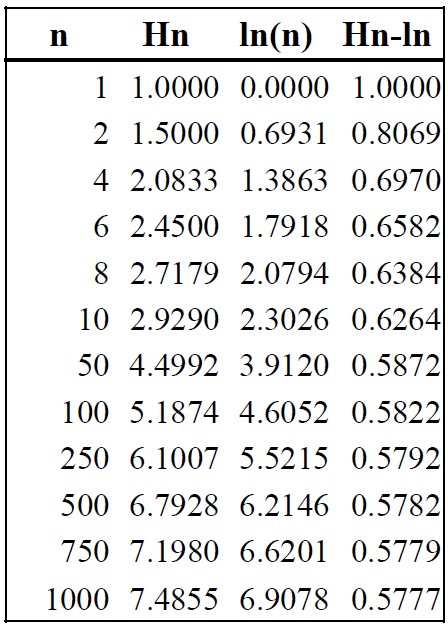
\includegraphics[scale=0.5]{Table of Euler Gamma Values more values.jpg}
    \caption{\textcolor{gray}{Table of Estimated Values of Eulers constant using a limit calculation: $\lim_{n\lra\infty}(\sum_{k=1}^{n}\frac{1}{k}-ln(n))$}}
    \label{fig:galaxy}
\end{figure}
\FloatBarrier
\begin{figure}[htp]
    \centering
    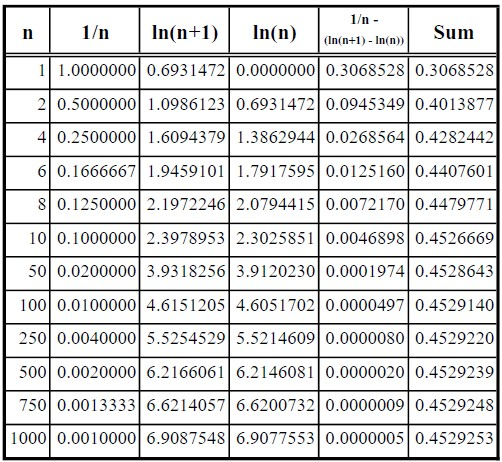
\includegraphics[scale=0.65]{table2 of euler gamma .jpg}
    \caption{\textcolor{gray}{Table of Estimated Values of Eulers constant using sum of the difference between $\frac{1}{n}-(ln(n+1)-ln(n))$ (dark shaded areas summed up)}}
\end{figure}




\section{Notes for draft ONLY May be left out of final version}
$ln(n) = \int_1^n \frac{1}{x}dx$\\
$\int_1^2 \frac{1}{x}dx+\int_2^3 \frac{1}{x}dx+...+\int_{n-1}^n \frac{1}{x}dx$\\
$\lim_{n\lra\infty}(\sum_{k=1}^{n} \frac{1}{k} + \sum_{k=1}^{n-1} \int_k^{k+1}\frac{1}{x}dx)$\\
End at $-n-1$ because final integral ends at $n$.\\
$\lim_{n\lra\infty}(\sum_{k=1}^{n-1} (\frac{1}{k} - \int_k^{k+1}\frac{1}{x}dx)+\frac{1}{n})$\\
$\leq \lim_{n\lra\infty}(\sum_{k=1}^{n-1} (\frac{1}{k} - \frac{1}{k+1})+\frac{1}{n})$\\
Because we have a monotonically decreasing function we can say this.\\
Unit interval (length one), replace $\frac{1}{x}$ with minimum value and since we are subtracting $\frac{1}{x+1}$ will be larger.\\
$\leq \lim_{n\lra\infty}(\sum_{k=1}^{n-1} (\frac{1}{k} - \frac{1}{k+1})+\frac{1}{n})=\lim_{n\lra\infty}(\sum_{k=1}^{n-1}(1-\frac{1}{2})+(\frac{1}{2}-\frac{1}{3})+(\frac{1}{n}-\frac{1}{n-1})+(\frac{1}{n}) = 1$ 
\begin{figure}[htp]
    \centering
    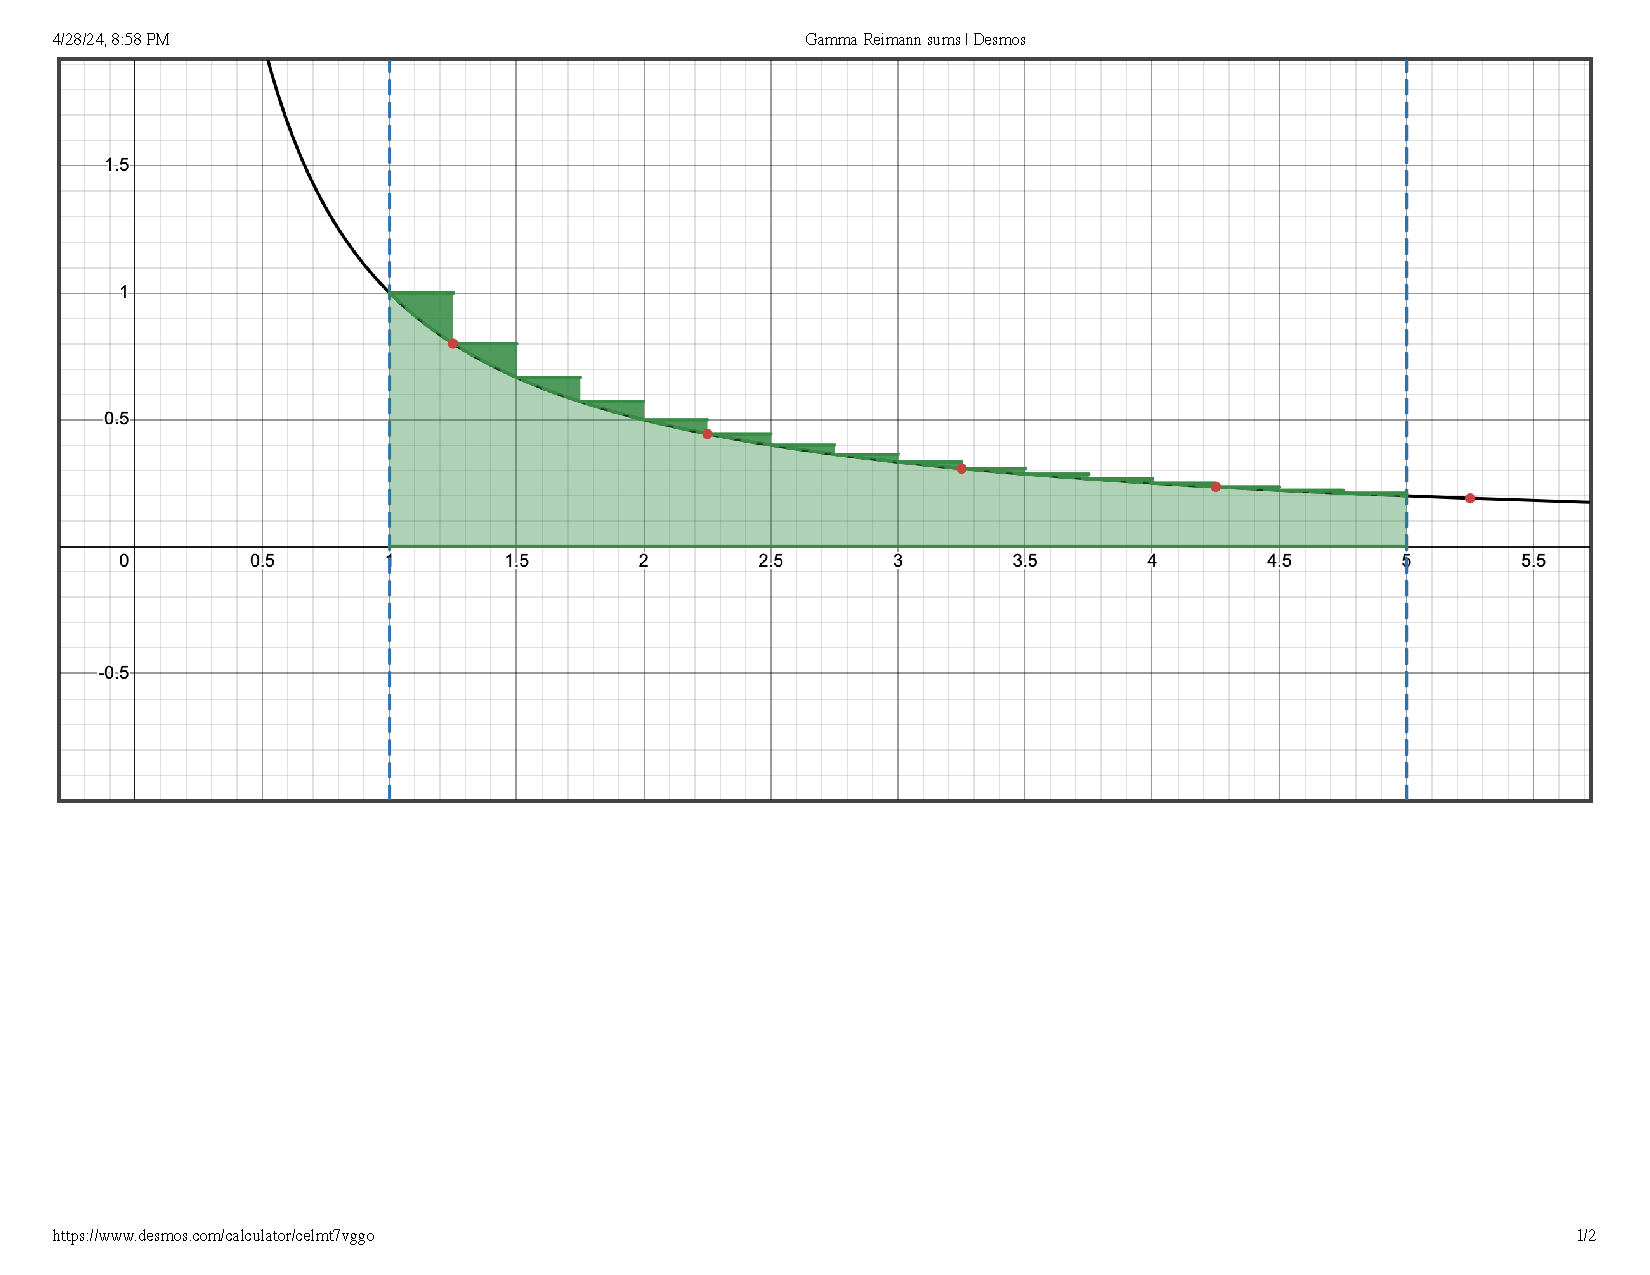
\includegraphics[scale=0.5]{Gamma Reimann sums _ Desmos.pdf}
    \caption{$\textcolor{OliveGreen}{Left\  Handed\  Riemann\  Sum\  of\  f(x)=\frac{1}{x}}$}
    \label{fig:Riemann Sums}
\end{figure}
The integral of each unit value n
$f(x)=\frac{1}{x}$\\
$ln(n) = \int_1^n \frac{1}{x}dx$\\
$\int_1^2 \frac{1}{x}dx+\int_2^3 \frac{1}{x}dx+...+\int_{n-1}^n \frac{1}{x}dx$\\
$0 < S_n=1+\frac{1}{2}+\frac{1}{3}+...\frac{1}{n}-ln(n)$\\
$(\int_1^2 \frac{1}{x}dx+\int_2^3 \frac{1}{x}dx+...+\int_{n-1}^n \frac{1}{x}dx)-(\int_{n-1}^n \frac{1}{x})$\\

Its decreasing so the function is less than the left end point.

Another way to consider this is that When we integrate $\frac{1}{x}$ this represents $\int_{n}^{n+1} \frac{1}{x}dx$ or:
$$ln(n+1)-ln(n)$$
$$\frac{ln(n+1)}{ln(n)}$$
The dark green area then represents the region represented by the function $\frac{1}{n} - \frac{ln(n+1)}{ln(n)} $  
\\Said differently the dark green area represents the unit value of $\frac{1}{x}$ minus the area under the curve of $\frac{1}{x}$ which can be represented by $\int_{n}^{n+1} \frac{1}{x}dx)$.
Figure 2 shows us graphically that $\int_n^{n+1} \frac{1}{x}dx$ will always be larger than $\frac{1}{n+1}$. This shows that $\frac{1}{x}$ is decreasing and left Riemann sum is an over estimate. This means $((-1)(\frac{1}{n+1})+\int_{n}^{n+1} \frac{1}{x}dx)$ will always be greater than $0$.
This confirms that $S_n-S_{n+1}$ will always be $>0$. We have shown that $S_n$ is monotonically decreasing.\\

\end{document}
